\documentclass[halfparskip]{beamer}


\mode<presentation>
{
  \usetheme{CambridgeUS}
  \usecolortheme{crane}
 
  \setbeamercovered{transparent}
}


\usepackage[ngerman]{babel}
\usepackage{enumitem}
\usepackage[T1]{fontenc}
\usepackage{graphicx}
\usepackage[utf8x]{inputenc}
\usepackage{lmodern}
\usepackage{tabularx}

\title{Crawling von Datenschutzerklärung-Historien}
\subtitle{Zwischenpräsentation}

\author[AP, JHD, SK]{Alexander Prull, Jörn-Henning Daug, Simon Kaleschke}

\institute{Universität Leipzig}

\date[16. 12. 2016]{16. Dezember 2016}

\subject{Crawling von Datenschutzerklärung-Historien}

\AtBeginSubsection[]
{
  \begin{frame}<beamer>{Gliederung}
    \tableofcontents[currentsection,currentsubsection]
  \end{frame}
}

\begin{document}

\begin{frame}
  \titlepage
\end{frame}

\begin{frame}{Gliederung}
  \tableofcontents
\end{frame}

\section{tmcrawl}
\subsection{Projektbeschreibung}
\begin{frame}{Projektbeschreibung}
	\begin{block}{Motivation}
	\begin{itemize}[label=$\bullet$]
	\item Aktuell geltende DSEs analysieren.
	\item Die Entwicklungsgeschichte von DSEs betrachten.
	\item Trends und Veränderungen beobachten.
	\end{itemize}
	\end{block}
	\begin{block}{Aufgaben}
		\begin{itemize}[label=$\bullet$]
			\item DSEs (täglich) extrahieren.
			\item Diese geeignet anzeigen.
			\item Unterschiede über Zeit darstellen.
		\end{itemize}
	\end{block}
	{\tiny DSE = Datenschutzerklärung}
\end{frame}

\subsection{Lösungsansatz}
\begin{frame}{Lösungsansatz}
	\begin{block}{Aufteilung}
		\begin{itemize}[label=$\bullet$]
			\item Extraktion: Ruby, XPath, SQLite.
			\item Backend: Java, REST-Services.
			\item Frontend: HTML5, CSS3, JavaScript, AngularJS, Bootstrap.
		\end{itemize}
	\end{block}
	\begin{block}{Arbeitspakete}
		\begin{itemize}[label=$\bullet$]
			\item Recherche (100 \%)
			\item Grundgerüst (80 \%)
			\item Feinschliff (0 \%)
		\end{itemize}
	\end{block}
\end{frame}

\subsection{Softwarearchitektur}
\begin{frame}{Extraktion}
	\centering
	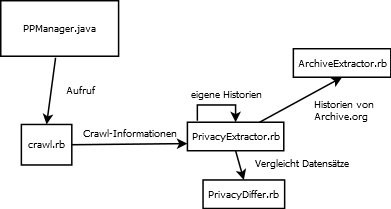
\includegraphics[scale=0.75]{extraction.png}
\end{frame}
\begin{frame}{Backend}
	\centering
	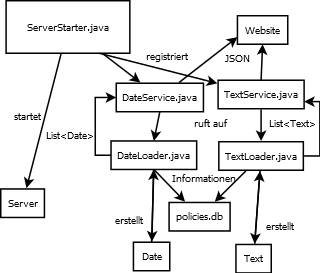
\includegraphics[scale=0.75]{backend.png}
\end{frame}
\begin{frame}{Website}
	\centering
	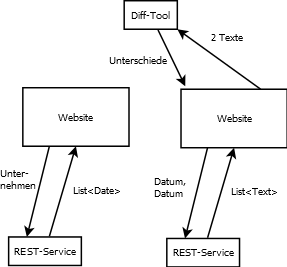
\includegraphics[scale=0.75]{frontend.png}
\end{frame}

\end{document}
